%%%%%%%%%%%%%%%%%%%%%%%%%%%%%%%%%%%%%%%%%%%%%%%%%%%%%%%%%%%%%%%%%%%%%%%%%%%
%%%%%%%%%%%%%%%%%%%%%%%%%%%%%%%%%%%%%%%%%%%%%%%%%%%%%%%%%%%%%%%%%%%%%%%%%%%
\section{Design and Principles of Recoil Separators}
% Experimental requirements, theory of separators, figures of merit
\label{emsep}

In this section we will present the equations for the motion of charged particles in magnetic and electric fields before discussing the types and design of ion-optical elements required in different designs of recoil separators, as well as exploring some of the rigidity and performance regimes for astrophysically important radiative capture reactions. 

For a recoil separator to function, it in principle has to induce a spacial separation between unreacted beam and recoil particles of different mass but similar momentum. In addition, it has to accept recoils with divergent angles with respect to the beam axis. In almost all cases discussed in this paper polarized beams are not used, therefore recoils are uniformly distributed in azimuthal angle, $\phi$. 
Thus in order for recoils to be separated, they must be brought to a focus in a mass-dispersed plane at some point. Due to the typical rigidities experienced in inverse kinematics at astrophysically-relevant energies, magnetic elements are required to provide the focusing. Electrostatic elements or combined electrostatic and magnetic elements can be used in addition to these to provide mass dispersion or beam rejection.  

The motion of a charged particle (with charge $q$) in external electromagnetic fields $\vec{E}$ and $\vec{B}$  is governed (non-relativistically) by the Lorentz force equation:

\begin{equation}
\vec{F}=q(\vec{E}+\vec{v}\times\vec{B})
\end{equation}   

where $\vec{v}$ is the instantaneous particle velocity. 

%%%%%%%%%%%%%%%%%%%%%%%%%%%%%%%%%%%%%%%%%%%%%%%%%%%%%%%%%%%%%%%%%%%%%%%%%%%
\subsection{Ion Optical Elements}

%%%%%
\subsubsection{Magnetic elements -- focussing and momentum/charge dispersion}\label{magel}

\small
\begin{itemize}
\item What are the necessary equations to present?
\item path of a charged particle in a magnetic field
\item image/object relationship
\item typical field strengths
\item double focussing, sextupole correction
\item its function as a momentum filter in our application means that we use it as a charge state filter because beam and reaction recoil have very similar central momentum
\item give equation for position of charge states blocked by slits
\end{itemize}
\normalsize

Magnetic quadrupoles are required in order to produce foci for the transported ions in the separator. This is usually achieved via doublets or triplets, providing net focussing in both the horizontal and vertical planes. While doublets are suitable for the bulk of the focussing, triplets may be required prior to a focus with more stringent requirements, such as an achromatic focus. This is due to the fact that in doublets changes in field strength in one axis might introduce undesirable changes in the other axis. Quadrupoles have focal lengths that are energy dependent in genera. l  

In addition, beam-target and recoil-target interactions will result in a distribution of charge-states being propagated through the separator. In order to bring the recoils to a unique mass-dfocus   

An ion moving in a uniform magnetic field follows a circular path, the radius of which is proportional to its  momentum.  The magnetic rigidity, the momentum $p$ divided by the ion charge $q$, is proportional to the product of $\rho$ the radius of curvature and $B$ the magnetic field, so ions of differing magnetic rigidity will be deflected through differing bend angles  when passing through a dipole magnet.  The reaction products and beam ions having overlapping values of momentum, a magnetic dipole by itself is ineffective as a mass separator.  However, it can be used to separate ions in a low-energy tail of the beam, which might be transmitted by electric field devices.

%%%%%
\subsubsection{Electrostatic elements}

\small
\begin{itemize}
\item path of a charged particle in an electrostatic field
\item typical necessary field strength/curvature for our application
\item focussing issues
\item acts as an energy filter
\item where does the not transmitted beam/charge states end up (split electrode approach, gridded possibility?)
\end{itemize}
\normalsize

A cathode and anode in the form of segments of concentric cylinders can produce a radial electric field which has constant magnitude $\mathcal{E}$  at a constant distance from the axis of the cylinders.   Ions having a suitable electric rigidity, the product of momentum $p$ and velocity $v$ divided by the charge $q$, can travel at a constant radius through the device.   Such an electrostatic dipole will deflect reaction products and beam ions through different angles due to their different velocities.  However, a low-energy tail of the beam, in a lower charge state and having the same electric rigidity as the reaction product, will not be separated.   This short-coming can be remedied by combining a magnetic dipole and electrostatic dipole in such a way that a subsequent angular focus is also a focus in ion energy but is dispersed according to ion mass.  

The required electrostatic fields are of order megavolts per metre.   Extensive measures, such as polishing the electrodes to a mirror finish, are required to prevent voltage breakdowns.   Because an electrostatic dipole must deflect desired particles through a permanently-fixed angle,  an experiment  cannot be performed unless the requisite   electrode voltages can be achieved.

notes about conditioning....

%%%%%
\subsubsection{Combined crossed field (Wien) filter elements}

\small
\begin{itemize}
\item what conditions have to be met to transmit the recoils (E,B field selection, condition)
\item what is the equation which tells us where the not transmitted beam and other charge states end up
\item typical fields and dimensions for our application
\end{itemize}
\normalsize

In a Wien filter parallel flat electrodes between the poles of a magnet provide crossed electric and magnetic fields, $\mathcal{E}$ and $B$.      There is a certain ratio $\mathcal{E}/B$ which results in ions of velocity $v$  undergoing no deflection as they pass through the Wien filter, regardless of their momentum $p$ or charge $q$.    Accordingly, a Wien filter can be tuned to pass the desired reaction product straight through while deflecting beam ions.  Like the electrostatic dipole, it may pass beam particles in  a low-energy tail; unlike the electrostatic dipole, it  also allows   neutral particles to pass through.

Because it is  the ratio $\mathcal{E}/B$ which selects the velocity, a Wien filter may operate with reduced\ field strengths (and reduced mass resolving power)  in order to accommodate reaction products of high rigidity, or if there is a problem reaching the designed maximum electric field.    On the other hand, a Wien filter poses greater design problems, requiring careful shaping of both the electrodes and the magnet poles in order to achieve the desired field uniformities and to match fringe fields.

%%%%%%%%%%%%%%%%%%%%%%%%%%%%%%%%%%%%%%%%%%%%%%%%%%%%%%%%%%%%%%%%%%%%%%%%%%%
\subsection{Performance}

%%%%%
\subsubsection{Beam suppression}
Reaction yield and detector performance together define the requirements for beam suppression by the separator.    The most challenging reactions  may well call for suppression by 10 to 12 orders of magnitude.    Separator designs for fusion-evaporation reactions, with higher yields and larger beam-product mass differences, may not be the best models  for radiative capture experiments.   
    
 One class of potential background is the tail of a  distribution generated by many small interactions, such as multiple scattering or energy straggling in the target.    Typically, these distributions have a Gaussian shape near their maximum but after only a few  ``standard deviations" the distributions become dominated by single large-deviation interactions, such as nuclear scattering in the target.    More complicated to assess are single scatterings from residual gas somewhere within the separator.   Nevertheless, it may be possible to investigate by computer simulation whether  a proposed separator design is able to suppress such events.
 
  ``Black Swan" events pose the most difficult problem for the separator designer.   By definition extremely rare and hard to foresee,  they are not  amenable to realistic simulation by computer.   Typically, they may involve sequential scatterings from  solid surfaces inside the separator.   The ranges of beam ions in solids being on order 1--10~$\mu$m, the surface material and roughness at the micrometer scale play a big role: oblique incidence on a smooth surface should be avoided and if possible such surfaces should be masked.   The separator designer must look to defense in depth, with more beam suppression features than the minimum required for events of the first  class.

%%%%%
  \subsubsection{Figure of merit}
  Some specifications, taken in combination, impose minimum requirements on the strength and extent of electric and magnetic fields.   These are the mass resolving power ($P_\mathrm{m}$), the angular acceptance ($\Delta a$) and the maximum particle rigidity 
  ($\mathcal{R}_\mathrm{M}=p/q$ or $\mathcal{R}_\mathrm{E}=pv/q$).    
  Consider a source of ions (reactions in the target), a dispersive device  (radius of curvature $\rho$) and an image (focus) point.   The  trajectories of the ions having the extremes in initial angles will delimit an area ($A$)  in the bend-plane of the dispersive device.     To first order the resolving power is given by the linear magnification ($M$) of the image, the mass dispersion ($D$) and the transverse source size ($\Delta x$): 
  $P_\mathrm{m} = D/(M \cdot \Delta x) $. 
  It has long been known (see, for example, \cite{Wo71}) that source emittance and the resolving power can be related to properties of the dispersive device by
  \[ P_\mathrm{m}\  \Delta a\  \Delta x = A/\rho \]
  Recalling that 
  $\mathcal{R}_\mathrm{M}=\rho \ B$ and $\mathcal{R}_\mathrm{E}=\rho \ \mathcal{E}$,  we obtain  figures of merit 
  \[ P_\mathrm{m}\  \Delta a\  \Delta x \ \mathcal{R}_\mathrm{M} = A \cdot B \]
   \[P_\mathrm{m}\  \Delta a\  \Delta x \ \mathcal{R}_\mathrm{E} = A \cdot \mathcal{E} \]
   That is, to achieve a certain figure of merit it is necessary to have a certain minimum product of field strength and area.  For an electrostatic device it may be convenient to use the length of electrodes and the gap between them as a proxy for the area $A$.  Then, the figure of merit becomes $L\cdot\Delta V$, where $L$ is the length of the electrodes and $\Delta V$ is the voltage difference between them.

%%%%%
\subsubsection{Additional factors} 
  Windowless targets either extended gas cell or gas jet, can impose major constraints on separator design.  Tubes between differential pumping stages may limit the convergence of incoming beam and consequently limit how small the beamspot  can be made at the target.  Pumping stages may set a minimum distance from target to the first focusing element.

Detectors of the heavy reaction product may have a maximum counting rate for optimum resolution, requiring a matching minimum beam suppression factor for the separator.   The detector may be limited in size, requiring a correspondingly small envelope of trajectories.    Good energy resolution or particle identification in a detector may permit a higher rate of beam leakage through the separator.

 The space   for the separator may be limited or the wrong shape if the experimental area was designed for the needs of earlier experiments.   Dipoles, quadrupoles  or Wien filters from elsewhere  may be available for use.  Finally,  funds for the project may be limited.   

%%%%%%%%%%%%%%%%%%%%%%%%%%%%%%%%%%%%%%%%%%%%%%%%%%%%%%%%%%%%%%%%%%%%%%%%%%%
\subsection{Gas targets}\label{gastarg}

%%%%%
\subsubsection{Windowless targets and differential pumping}


For our purpose of measuring proton or alpha radiative capture in inverse kinematics, a hydrogen or helium gas target is required which has sufficient density  to contain energetically the targeted resonance width or a sufficient direct capture interval to provide a measurable yield. Additionally, the uncertainty of a resonance position --- from transfer reaction measurements and nuclear mass information --- has to be taken into account. As the resonant yield is inverse proportional to the target stopping power it is also beneficial to avoid inactive nuclei in its composition, {\it e.g.} a pure hydrogen target provides a factor 3--4 higher yield than a CH$_2$ foil target.  A gas target is also virtually indestructible and stable in its composition while in plastic foil targets the carbon to hydrogen ratio is known to change even under modest heavy ion beam flux of the order of $10^7 \unit{s^{-1}}$.\\
In order to achieve a target thickness of 10 keV (in the centre-of-mass system) with the light to medium mass ion beams in question at astrophysically relevant energies, a target number density of approximately $5\cdot10^{18} \unit{nuclei/cm^2}$ of hydrogen is required. To provide unimpeded beam and recoil transmission, the gas cannot be confined by foil windows, leaving as the only possible approach the use of a windowless, differentially pumped gas target. The gas pressure necessary to achieve the required target number density is given by the formula \cite{rolf88} 
\begin{equation}
n_A = 9.66\cdot10^{18} x \nu \frac{p}{T} \mathrm{[1/cm^2]}
\end{equation}
with $x$ the target length in cm, $\nu$ the number of atoms per molecule, $p$ the pressure in Torr, and $T$ the temperature in K.\\
It should be noted that the target length needs to be kept small ($<$ 10--15 cm) in order not to significantly increase the acceptance requirements for the recoil separator. The windowless approach means that a target pressure of a few torr needs to be maintained in the gas cell, but a reduction to the order of $10^{-6} \unit{Torr}$ achieved over several gas flow limiting apertures and pumping stages is necessary to allow connection to the accelerator and separator. On the accelerator side the dimensions of these apertures are defined typically by the beam dimensions, while on the separator side the reaction recoil cone needs to be accommodated. Therefore, it is preferable to compress the length of the differential pumping stages as much as possible to allow for smaller aperture sizes. A typical pumping scheme is depicted in Fig. \ref{fig:dragon_pumping}.
\begin{figure}
\resizebox{0.9\columnwidth}{!}{
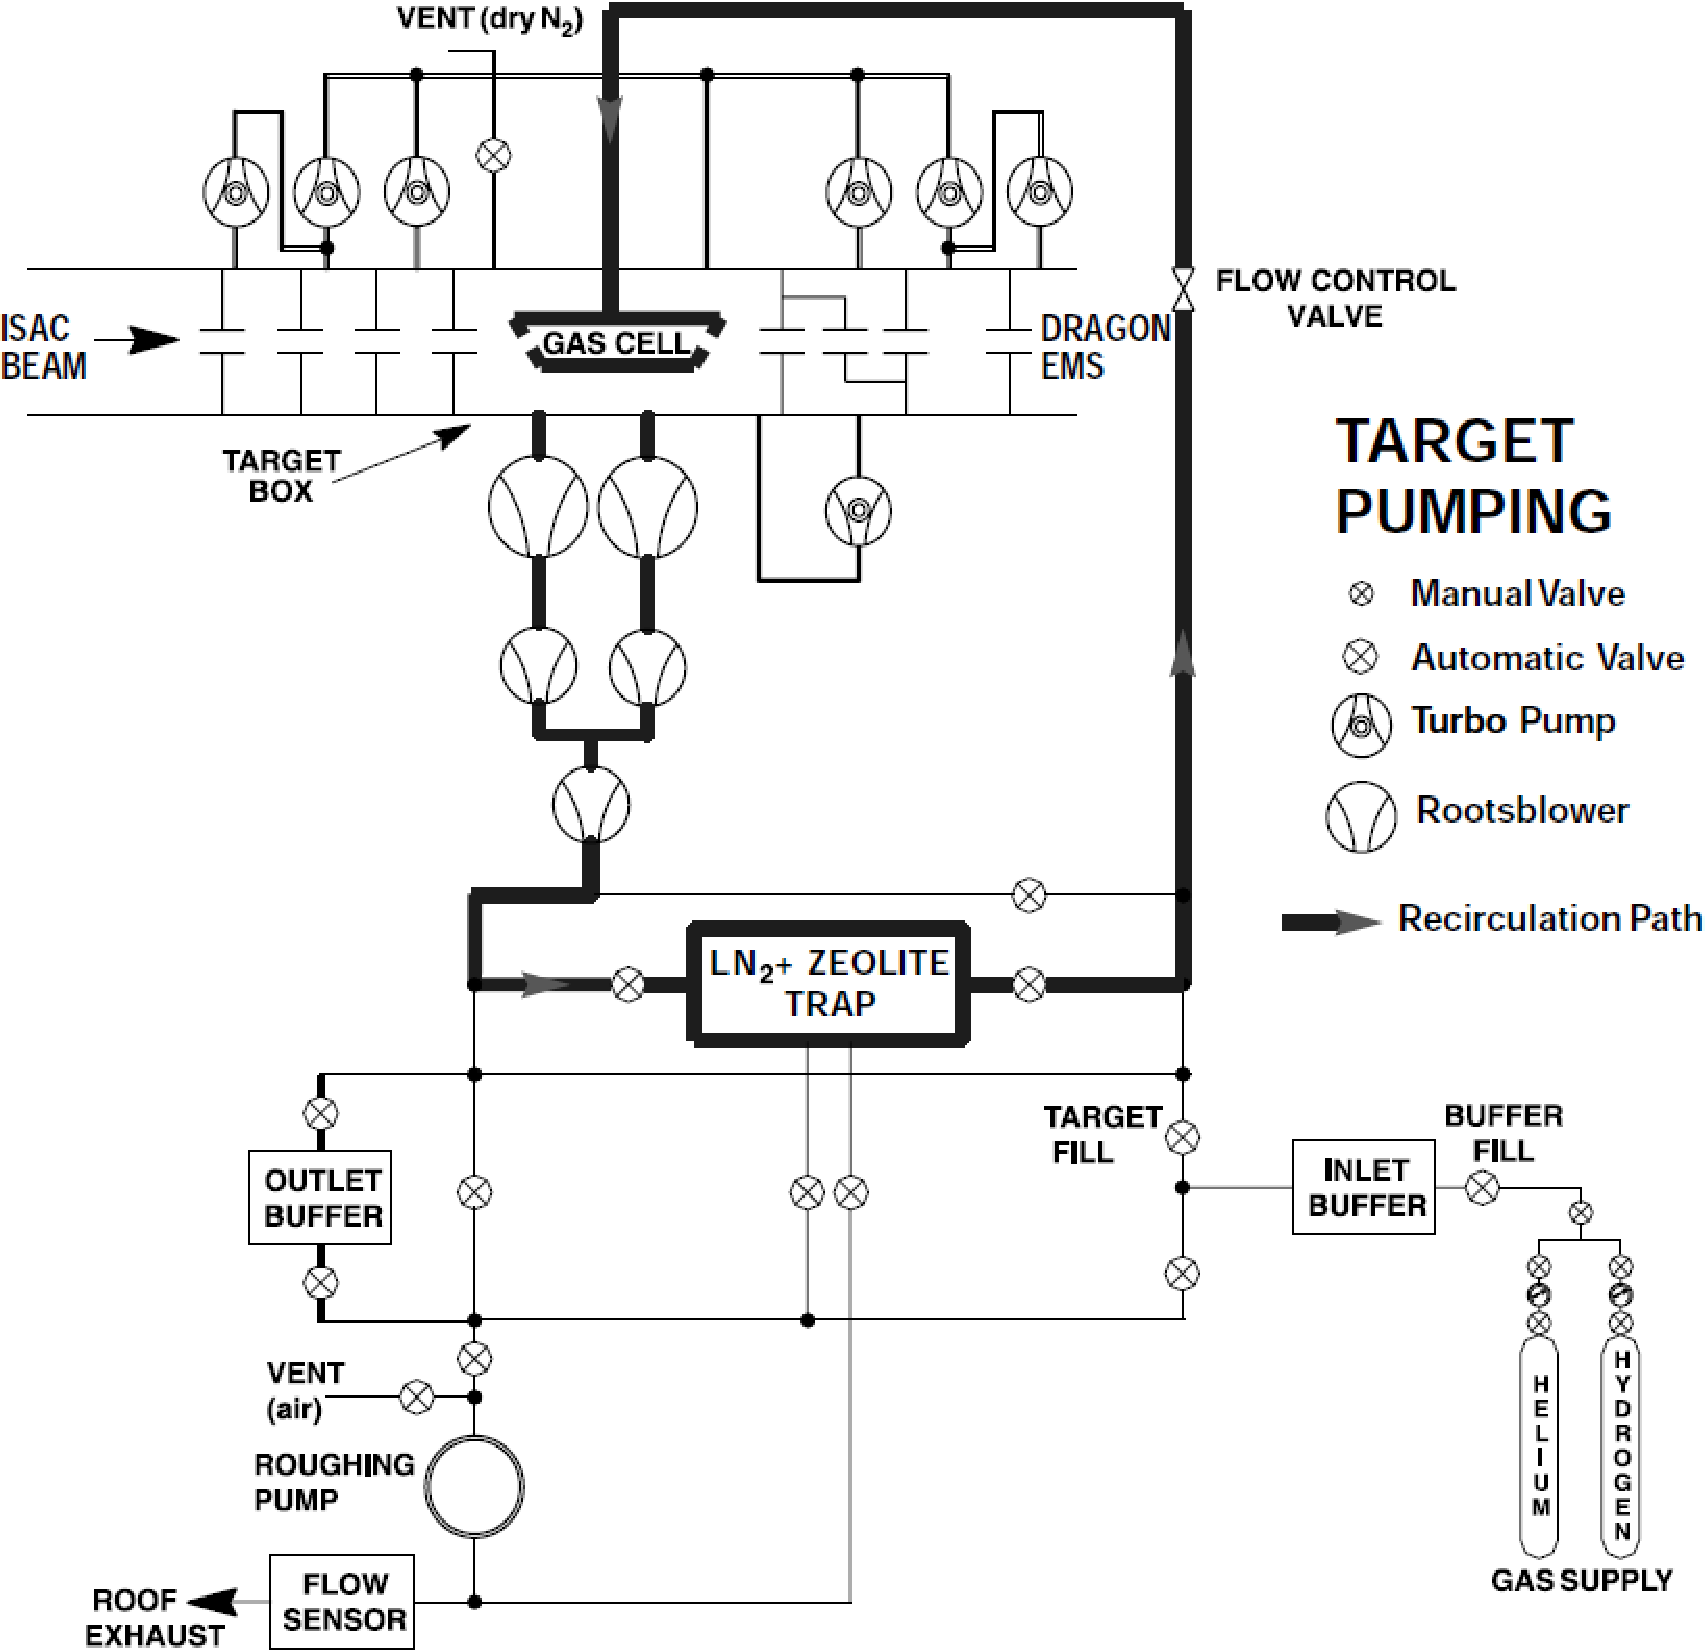
\includegraphics{Hutcheon03_Fig5_DRAGON-gastargetpumps}
}
%\vspace{5cm}       % Give the correct figure height in cm
\caption{DRAGON gas target pumping scheme. Taken from \cite{hutc03b}.}
\label{fig:dragon_pumping}
\end{figure}
\emph{[Figure of pumping scheme]} \\
For the extraction of a cross section or resonance strength from the measured yield we require knowledge of the stopping power of the heavy ions in hydrogen or helium. While these are typically taken from the widely used SRIM code \cite{zieg}, recent experiments \cite{grei04} have shown deviations of the order of 20--30 \% from the semi-empirical values. Therefore, direct measurement of the respective stopping power should, where possible, be preferred. Additionally, angle and energy scattering of the beam and recoils on their way through the target gas need to be estimated and taken into account in the calculation of the required recoil separator acceptance. While the ions pass the gas they also undergo charge-changing collisions. If the target is thick enough, an equilibrium charge state distribution is achieved (semi-empirical description available in {\it e.g.} \cite{liu03}). However, if the reaction recoil originates from the downstream side of the gas target, the remaining gas track length is not sufficient to reach this equilibrium, and it is advisable to obtain the charge state distribution by tuning the recoil separator for measurements of the several charge states expected to be most abundant.\\
Especially for the astrophysically most important reactions \nuc{12}{C}\reac{\alpha}{\gamma}\nuc{16}{O} and \nuc{15}{O}\reac{\alpha}{\gamma}\nuc{19}{Ne}, the recoil cone angles are quite demanding on separator acceptance. In order not to alleviate \emph{[alleviate? do you mean aggravate?]} the problem through the use of an extended gas target length of 5 -- 10 cm, recent discussions propose the use of a gas jet target with approximately 4 -- 5 mm jet diameter matched to the dimension of the incoming ion beam. As can be seen in the pumping scheme \emph{[gas jet target pumping scheme figure]} for an appropriate gas jet target ($\approx 5\cdot10^{18} \unit{cm^{-1}}$ areal density), such a setup (which is in its early construction phases for deployment at Oak Ridge National Laboratory) requires significantly more powerful pumping stages as well as expensive gas compression and cleaning.\\
 

\small
\begin{itemize} 
\item What are the advantages of using a differentially pumped windowless gas target?
\item for our purpose H and He targets best solution as he not available implanted in sufficient densities; H possibles but about factor 4 yield advantage due to 1/stopping term in resonant yeild equation
\item also indestructible and stable in composition (plastic foils change and have current limit)
\item windows are detrimental to recoil transmission, therefor windowless, differentially pumped approach ideal for our application
\item what thickness to chooses: resonance width (usually small) + uncertainty in resonance position (info from transfer reactions plus knowledge of masses of reaction partners of order a few keV) follows target thickness of about 10 kev in CM system is useful leading areal target densities aspired of 5E18 1/cm2
\item at 7-8 Torr achieved with about 10 cm length
\item give equation from Rolfs for gas target density
\item  length of target determines origin of recoil; needs to be matched with acceptance of the recoil separator (shorter is better); some reactions would benefit from gas jet which is however technically more challenging due to the large gas flow rates involved.
\item Gas flow limiting apertures need to be matched to the heavy (radioactive) ion beam properties and the nuclear reaction recoil cone angle
\item we need to know stopping powers; found differences to SRIM of the order of 20-30% when we measured ourselves
\item energy and angle scattering needs to be estimated and included in acceptances; not well known
\item charge state distributions, often equilibrium not achieved; preferably to be measured in experiment
\end{itemize}
\normalsize

%%%%%
\subsubsection{Extended length targets}

%%%%%
\subsubsection{Gas jet targets}
